\documentclass[conference]{IEEEtran}
\IEEEoverridecommandlockouts
\usepackage{cite}
\usepackage{amsmath,amssymb,amsfonts}
\usepackage{graphicx}
\usepackage{textcomp}
\usepackage{xcolor}
\usepackage{booktabs}
\usepackage{siunitx}
\usepackage{url}
% generated by analysis/paper_numbers.py -- do not edit
\newcommand{\bpDistance}{2}
\newcommand{\bpTpass}{2}
\newcommand{\bpTstar}{4}
\newcommand{\bwHwLoneMean}{$+$0.052}
\newcommand{\bwIdealLoneMean}{$+$0.053}
\newcommand{\chiMaxRecord}{96}
\newcommand{\chshS}{2.733}
\newcommand{\chshSig}{0.032}
\newcommand{\chshZ}{22.7}
\newcommand{\coreSecMax}{146}
\newcommand{\corrRmsHw}{0.119}
\newcommand{\corrRmsIdeal}{0.166}
\newcommand{\corrRmsIndep}{0.016}
\newcommand{\corrRmsNoisy}{0.114}
\newcommand{\costMaxS}{18}
\newcommand{\costPjFifty}{1.0}
\newcommand{\costPjSevenSeven}{1.5}
\newcommand{\dLtwoOrders}{11.3}
\newcommand{\dampNineK}{15.5}
\newcommand{\dampTenK}{1.9}
\newcommand{\envMatchAll}{every}
\newcommand{\ghzF}{0.055}
\newcommand{\ghzFsig}{0.019}
\newcommand{\ghzTwo}{0.946}
\newcommand{\ghzTwoX}{0.144}
\newcommand{\ghzTwoZZ}{0.802}
\newcommand{\mFourTwentyFourRetainPct}{5.0}
\newcommand{\motileMax}{1.965}
\newcommand{\motileMin}{1.959}
\newcommand{\nHwProjects}{three}
\newcommand{\nHwRunFiles}{141}
\newcommand{\pjEntNat}{0.120}
\newcommand{\pjFiftyRetainPct}{5.8}
\newcommand{\pjSepNat}{0.899}
\newcommand{\qtChiLfour}{46}
\newcommand{\qtCostLfour}{101}
\newcommand{\qtCostLtwo}{5.0}
\newcommand{\qtDepthFloor}{113}
\newcommand{\qtDepthLone}{113}
\newcommand{\qtDivHw}{0.94}
\newcommand{\qtDivSim}{0.85}
\newcommand{\qtHwLoneMean}{$+$0.024}
\newcommand{\qtHwLtwoMean}{$-$0.104}
\newcommand{\qtIdealLoneMean}{$+$0.0008}
\newcommand{\qtIdealLtwoMax}{$-$0.132}
\newcommand{\qtIdealLtwoMin}{$-$0.183}
\newcommand{\qtZsim}{13.7}
\newcommand{\renderCellsP}{0.88}
\newcommand{\renderCellsQ}{151.7}
\newcommand{\renderCellsT}{135.4}
\newcommand{\renderDiamP}{0.88}
\newcommand{\renderDiamQ}{11.4}
\newcommand{\renderDiamT}{11.4}
\newcommand{\renderGlcmP}{0.88}
\newcommand{\renderGlcmQ}{246.5}
\newcommand{\renderGlcmT}{245.8}
\newcommand{\renderKsCrit}{0.32}
\newcommand{\renderMinP}{0.88}
\newcommand{\renderNq}{36}
\newcommand{\renderNt}{36}
\newcommand{\renderPairedMinP}{0.25}
\newcommand{\renderRoiP}{0.98}
\newcommand{\renderRoiQ}{131.6}
\newcommand{\renderRoiT}{131.8}
\newcommand{\renderVdtP}{0.98}
\newcommand{\renderVdtQ}{622.3}
\newcommand{\renderVdtT}{599.8}
\newcommand{\rollDepthIsa}{1616}
\newcommand{\rollExp}{4.4, 2.0, 1.2, 0.4}
\newcommand{\rollIdeal}{0.554, 0.247, 0.148, 0.051}
\newcommand{\rollMC}{200{,}000}
\newcommand{\rollN}{8}
\newcommand{\rollNoisy}{0.438, 0.254, 0.194, 0.114}
\newcommand{\rollObs}{1, 0, 5, 2}
\newcommand{\rollP}{1.7\times10^{-4}}
\newcommand{\rollPct}{0.022}
\newcommand{\rollTwoQIsa}{642}
\newcommand{\rollTwoQLogical}{104}
\newcommand{\scanChiA}{13}
\newcommand{\scanChiB}{45}
\newcommand{\scanChiC}{492}
\newcommand{\scanChiD}{n/a}
\newcommand{\scanChiE}{n/a}
\newcommand{\scanChiF}{256}
\newcommand{\scanT3chi}{482}
\newcommand{\scanT3max}{144}
\newcommand{\scanT3min}{42}
\newcommand{\scanTA}{0.11}
\newcommand{\scanTB}{0.51}
\newcommand{\scanTC}{68.53}
\newcommand{\scanTD}{$>1200$}
\newcommand{\scanTE}{$>1200$}
\newcommand{\scanTF}{66.08}
\newcommand{\scanTwoQA}{92}
\newcommand{\scanTwoQB}{138}
\newcommand{\scanTwoQC}{184}
\newcommand{\scanTwoQD}{n/a}
\newcommand{\scanTwoQE}{n/a}
\newcommand{\scanTwoQF}{240}
\newcommand{\seedElongKsIdeal}{0.033}
\newcommand{\seedElongKsIndep}{0.044}
\newcommand{\seedElongKsNoisy}{0.017}
\newcommand{\seedKsIdeal}{0.120}
\newcommand{\seedKsIndep}{0.085}
\newcommand{\seedKsNoisy}{0.073}
\newcommand{\seedKsPmax}{9.5\times10^{-113}}
\newcommand{\seedKsSplit}{0.010}
\newcommand{\seedKsSplitP}{0.18}
\newcommand{\seedN}{48{,}000}
\newcommand{\seedReproOk}{12}
\newcommand{\seedTiles}{12}
\newcommand{\seedVoxHw}{202.7}
\newcommand{\seedVoxIdeal}{174.3}
\newcommand{\seedVoxIndep}{220.9}
\newcommand{\seedVoxNoisy}{183.8}
\newcommand{\sigReduced}{$+$0.0042}
\newcommand{\surrDamp}{0.24}
\newcommand{\surrUnitaryCode}{0.92}
\newcommand{\surrUnitaryFixed}{$8\times10^{-14}$}
\newcommand{\swapDepth}{31}
\newcommand{\swapGens}{32}
\newcommand{\swapHw}{$+$0.040}
\newcommand{\swapIdeal}{$-$0.071}
\newcommand{\swapSignWrongPct}{72}
\newcommand{\telDepth}{9}
\newcommand{\telHwLedger}{$-$0.128$\pm$0.012}

% generated by analysis/paper_numbers.py -- do not edit
\newcommand{\teleportAuditCell}{SWAP ideal $-$0.071, hardware $+$0.040}
\newcommand{\teleportParagraph}{A teleported long-range CNOT on 104 qubits (logical depth 9) was compared with a SWAP ladder (depth 31) at distance 12. We replayed every SWAP-arm hardware generation exactly: beliefs rebuilt from the recorded frequencies, with the environment schedule matching the recorded one in every generation. The SWAP arm reads $+$0.040 on hardware where its ideal is $-$0.071; the sign is wrong in 72\% of 32 generations. The teleport arm reads $-$0.128$\pm$0.012 on hardware; its exact replay (mid-circuit measurement forces a per-shot simulation of 104 qubits) did not finish within our compute budget, so we report no ideal for it. The original write-up quoted an exact ideal of $-$0.29; its own script, rerun, gives a mean of $+$0.0042 on its reduced 18-qubit model with alternating sign. A depth comparison alone decides nothing; the exact replay does.}
\newcommand{\scanParagraph}{We measure the distance to L2 on two axes. \emph{Cost.} The most expensive exact reproduction of a hardware result in Table~\ref{tab:record} took 18~s, at most 146 core-seconds on eight cores. Taking $10^6$ core-years ($3.2\times10^{13}$ core-seconds) as a conservative threshold for ``out of classical reach'', the record sits 11.3 orders of magnitude below it (Fig.~\ref{fig:map}). For the genealogy family this distance does not shrink with better hardware, because $\chi$ stays 2 at every width. \emph{Depth.} The QCA is the only family with non-Clifford coupling on a lattice with loops. On the live 23-site region, belief propagation with $\chi\le16$ converges up to depth $t=3$ and fails from $t^*=4$. Hardware passed its pair witness at $t=2$, so the depth distance is 2 steps. Failure of belief propagation is not classical hardness: exact MPS reproduces the same 23 sites at $t=4$ in 68.53~s ($\chi=492$). Exact cost does rise steeply with width and depth (Table~\ref{tab:scan}): at 40 or more sites, $t=3$ costs 42 to 144~s ($\chi$ up to 482) and $t=4$ did not finish within 1200~s and 20~GB at any width. That is the direction in which an L2 candidate could appear. It needs a passing witness at the same width and depth, and today the witness at $t=2$ passed on one of four pairs.}
\newcommand{\ctParagraph}{The live run rolled twelve tumours (8 independent words and two sibling pairs) in one job on \texttt{ibm\_marrakesh}, with a CHSH test in the same job: $S=2.733\pm0.032$ (2048 shots per setting), 22.7$\sigma$ above the local bound. Every case is therefore P-L0. Each grown tumour starts from one Z snapshot of a 23-site QCA measured in a second job, whose pair witness passed marginally. We compared three levels with classical twins. \emph{Roll.} The independent size draws were (1, 0, 5, 2) for the bands $<6$, 6--8, 8--20 and $>20$~mm, against (4.4, 2.0, 1.2, 0.4) expected under the rulebook (Table~\ref{tab:roll}). Against 200{,}000 classical cohorts drawn from the same rulebook this gives $p=1.7\times10^{-4}$ (G statistic), and the joint log-likelihood falls at percentile 0.022\%. The 9-qubit roll compiles from 104 to 642 two-qubit gates (depth 1616); simulated Heron noise moves the ideal size mix (0.554, 0.247, 0.148, 0.051) to (0.438, 0.254, 0.194, 0.114), the same direction as the hardware. \emph{Seeds.} For each tile we compared the 48{,}000 hardware snapshots per arm with an ideal sampler of the same circuit, a noisy sampler and independent coins with the hardware marginals (Fig.~\ref{fig:twin}a). Hardware split halves agree (seed-size KS $D=0.010$, $p=0.18$); hardware differs from the ideal ($D=0.120$), noisy ($D=0.073$) and independent ($D=0.085$) twins, all $p\le9.5\times10^{-113}$. The mean pair-correlation RMS is 0.119 on hardware, 0.166 ideal, 0.114 noisy and 0.016 for independent coins. The seed structure comes from correlations that any classical sampler given the joint distribution reproduces, and that a marginals-only sampler loses. All 12 of 12 stored seeds were regenerated from the recorded hardware bits. \emph{Rendered nodules.} Four replicate cohorts per arm, each grown and rendered into the same Siemens-scanner host, gave 36 quantum-seeded and 36 twin-seeded nodules (Fig.~\ref{fig:twin}b). No feature differed: KS $p\ge0.88$, paired per-tile Wilcoxon $p\ge0.25$. Baseline diameter is equal by construction, because growth targets the rolled size. At these sample sizes the test detects $D\ge0.32$; smaller differences are not excluded.}
\newcommand{\ruleParagraph}{The case study separates what the quantum computer adds from what it costs. The Bell test certifies that the draw was not chosen. After rendering, the content cannot be told from its classical twin. Sampling the rulebook directly on hardware distorted the medical statistics ($p=1.7\times10^{-4}$). The rule that follows: certify the seed on the quantum computer, then sample the content classically from it, for example with a deterministic random bit generator keyed by the certified bits~\cite{barker2015}. The classical twin then \emph{is} the generator. The rulebook is reproduced up to sampling noise, and the job identifier, the $S$ value and the seed hash travel with every case as its replayable record. Quantum structure, where wanted (correlated sibling lesions, lineage-shaped seeds), is added only with a passing witness in the same job and labelled P-L1.}
\newcommand{\conclusionParagraph}{Today's quantum computers can do one thing for medical imaging that classical generators cannot: certify that synthetic validation cases were not chosen. In our live cohort the Bell value was $S=2.733$, 22.7$\sigma$ above the local bound. Every case is replayable from its seed, and its content cannot be told from a classical twin. The design rule is to certify the seed on the quantum computer and sample the content classically. From there the road to more complex quantum-native content has three further layers, each with a pass criterion: correlated families from one entangled lineage, compressed growth models, and seed structure beyond classical reach. The nearest open cell is the QCA at depth four and forty or more sites, which exact classical simulation on one machine did not finish. Quantum simulation of life itself is not on that road yet: every faithful circuit we ran was reproduced classically in at most 18~s. Certified, not superior, is the honest starting point, and it is already useful.}
\newcommand{\figOneCaption}{Every hardware result in our record, placed by its margin above the classical bound of its witness (vertical, symmetric log scale; marker = witness rung, colour = project) and by the measured cost of reproducing it exactly on one eight-core machine (horizontal, core-seconds). Dashed lines: cost tiers. Shaded: alive and beyond $10^6$ core-years, the region an L2 claim needs; it is empty. Lower strip: the QCA family in simulation only (exact MPS, ideal) by patch size and depth; arrows mark cells that did not finish within 1200~s and 20~GB.}
\newcommand{\figTwoCaption}{Classical-twin test of the procedurally generated CT nodules. (a)~Seed size over 48{,}000 QCA snapshots per arm: hardware, an ideal classical sampler of the same circuit, a noisy sampler (FakeMarrakesh noise model) and independent coins with the hardware marginals. (b)~Rendered nodules from four replicate cohorts per arm, quantum-seeded ($n=36$) vs twin-seeded ($n=36$), standardised per feature; two-sample KS $p$ per feature.}


\begin{document}

\title{Certified, Not Superior: What Quantum Computers Can Honestly Generate, from Artificial Life to Synthetic CT}

\author{
\IEEEauthorblockN{Peter Jas}
\IEEEauthorblockA{\textit{affiliation (to be added)}\\
City, Country\\
email address or ORCID}
}

\maketitle

\begin{abstract}
Synthetic cases used to validate medical imaging AI are only useful as evidence if their origin can be proven:
nobody picked them, anyone can replay them, and they follow published clinical statistics. Today's quantum
computers can already do this job, and it needs no speed-up. On a 156-qubit IBM Heron processor we rolled a cohort
of synthetic lung tumours together with a Bell test in the same job, which scored \chshS{}, \chshZ{} standard
deviations above the classical limit, then grew the tumours and rendered them into a real chest CT from a Siemens
scanner. Every case carries its job identifier, its Bell value and a replayable seed. A classical twin of the
generator shows that the content itself is indistinguishable: across \renderNq{} quantum-seeded and \renderNt{}
twin-seeded nodules no image feature differed. The design rule is to certify the seed on the quantum computer and
sample the content classically, because sampling clinical statistics directly on noisy hardware distorted them. We
lay out the road from certified generation to more complex quantum-native content in four measurable layers. We
also state what is not worth pursuing yet. In \nHwRunFiles{} hardware runs, most of them quantum life simulations
on up to 108 qubits, every result was reproduced exactly by one classical machine in at most two minutes, so
quantum life simulation is not yet a route to better medical prediction.
\end{abstract}

\begin{IEEEkeywords}
quantum computing, procedural content generation, synthetic CT, provenance, Bell test, quantum artificial life,
classical simulation, entanglement witness
\end{IEEEkeywords}

\section{Introduction}
Detection and segmentation models for medical images need test cases that real data covers poorly: tiny, faint or
juxtapleural nodules, rare scanners, controlled difficulty. Synthetic cases can fill that gap, but only if they are
credible evidence. Exact ground truth, no patient voxels in the generator and a traceable origin are the
requirements, and the last one includes a property that is easy to state and hard to prove: nobody chose the cases.
A Bell test certifies exactly that for random bits drawn in the same experiment~\cite{clauser1969,pironio2010}.
This gives quantum computers a medical job that exists today and needs no speed-up.

The surrounding field is crowded with stronger promises. Systematic reviews of quantum computing in biology find
almost no hardware execution at realistic scale and no demonstrated advantage~\cite{arcieri2026}, and frameworks for
judging advantage in biology and medicine show how far most proposals are from one~\cite{cordier2022}. We take a
constructive position and separate three things: what quantum computers can do for medical imaging now, the road
to more complex quantum-native content, and what is not worth pursuing yet. Each part rests on our own hardware
record: \nHwRunFiles{} hardware runs from \nHwProjects{} projects on two 156-qubit IBM Heron~r2 processors
(\texttt{ibm\_kingston}, \texttt{ibm\_marrakesh}) between July and October 2026. These are a quantum tree grown on up
to 108 qubits, a faithful rebuild of quantum artificial life scaled to 100 qubits, and a synthetic-CT pipeline. Earlier
runs on \texttt{ibm\_fez} were not retained and are not used.

\textbf{Contributions.}
(i)~Certified procedural generation of synthetic chest CT, measured end to end against classical twins, with a
provenance ladder and a design rule (Section~\ref{sec:pcg}, Fig.~\ref{fig:twin}).
(ii)~A road from certified seeds to quantum-native content in four layers, each with a pass criterion, and an
objective measure of the remaining distance to classical intractability (Section~\ref{sec:road}, Fig.~\ref{fig:map}).
(iii)~What does not work yet: for every hardware result of our life simulations, the exact classical reproduction
cost, nine checks learned from our own mistakes, and three structural reasons why faithful evolution circuits are
classically easy (Sections~\ref{sec:life} and~\ref{sec:easy}).

\section{What a quantum claim has to show}\label{sec:ladder}
Any distribution of measurement outcomes in a single basis can be reproduced by a classical sampler that is given
the same probabilities. Every readout that encodes biology or an image (cell counts, lineage sizes, tumour size,
voxels) is such a readout. A quantum claim therefore lives in correlations measured in more than one basis, in a
resource cost, or in a certificate. We use five claim levels:
\textbf{L0} provenance (a Bell test certifies that nobody chose the draw);
\textbf{L1} the generating state was entangled (a witness passed);
\textbf{L1$'$} a memory advantage of the quantum model of a stochastic process~\cite{gu2012};
\textbf{L2} the output distribution is hard to sample classically;
\textbf{L3} a useful computational advantage.
An entanglement witness is an observable whose expectation value is bounded for every separable state; a measured
violation proves entanglement without tomography~\cite{guhne2009}. The witnesses in our record fall on four rungs:
\textbf{W-a} a connected correlation compared with one chosen classical surrogate, which excludes only that
surrogate; \textbf{W-b} a two-qubit witness, here $\langle XX\rangle+\langle ZZ\rangle\le 1$ for separable pairs, or
pair negativity; \textbf{W-c} genuine multipartite entanglement, for example GHZ fidelity above $1/2$, which needs only
two measurement settings~\cite{toth2005}; \textbf{W-d} a Bell test, CHSH $S\le 2$ for local models. Entanglement is
necessary for classical hardness~\cite{jozsa2003,vidal2003} but not sufficient: GHZ states are maximally entangled
and classically trivial~\cite{gottesman1998}.

\section{Certified procedural generation of synthetic CT}\label{sec:pcg}
A content generator for validation data is judged on four properties: nobody chose the content, the same seed
replays the same content, the content follows a specification, and there is a record a reviewer can check. None of
the four needs L2, and L0 already delivers the first one with a certificate no classical generator can give.
We use a provenance ladder for generated content. \textbf{P-L0}: a Bell test in the same job certifies the draw.
\textbf{P-L1}: the job that produced the content also passed an entanglement witness. \textbf{P-L1$'$}: a compressed
generator. \textbf{P-L2}: content drawn from a distribution outside classical sampling reach. Every generated item
ships with a \emph{classical twin}, the same item produced by a classical sampler fed the same probabilities, so the
claim is always about the record and never about appearance. Earlier quantum procedural generation, such as quantum
blur~\cite{wootton2020}, made appearance claims. In our reproduction a classical Gaussian filter matched its output at
$r$ up to 0.99, and where it differed it scrambled coordinate bits non-physically.

\textbf{Pipeline.} The synthetic-CT pipeline rolls each tumour's size, type, margin and lobe from a published
rulebook encoded in a 9-qubit circuit, together with a CHSH test in the same job. It takes each tumour's seed shape
from one snapshot of a 23-site quantum cellular automaton (QCA) and grows it classically with a cellular
automaton~\cite{kansal2000}. Each nodule is then rendered into a public chest CT acquired on a Siemens
scanner~\cite{armato2011}, with that scanner's measured blur and noise. No patient voxels enter the generator.

\textbf{Case study.} \ctParagraph

\begin{figure*}[t]
\centering
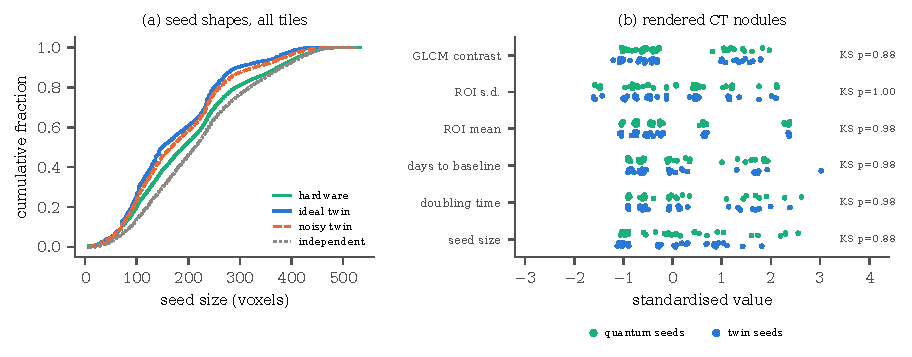
\includegraphics[width=\textwidth]{fig2_twin.pdf}
\caption{\figTwoCaption}
\label{fig:twin}
\end{figure*}

\begin{table}[t]
\centering
\caption{Size mix of the 9-qubit tumour roll: published rulebook, exact ideal simulation, simulation with a
Heron-class noise model (FakeMarrakesh) and the eight independent hardware draws of the live job.}
\label{tab:roll}
\small
\begin{tabular}{lrrrr}
\toprule
Size band & rulebook & ideal sim & noisy sim & hardware\\
\midrule
$<6$ mm & 0.550 & 0.554 & 0.438 & 1/8\\
6--8 mm & 0.250 & 0.247 & 0.254 & 0/8\\
8--20 mm & 0.150 & 0.148 & 0.194 & 5/8\\
$>20$ mm & 0.050 & 0.051 & 0.114 & 2/8\\
\midrule
shots or draws & -- & 100{,}000 & 100{,}000 & 8\\
\bottomrule
\end{tabular}

\end{table}

\textbf{Design rule.} \ruleParagraph

\section{The road to more complex systems}\label{sec:road}
Certified generation is the base layer. Each further layer adds one quantum ingredient and comes with a pass
criterion that the next hardware generation can check without new theory.

\textbf{Layer 1, certified seeds (P-L0): done.} Every case of the live cohort carries a Bell value of
$S=\chshS\pm\chshSig$ from its own job, a job identifier and a seed hash, and is replayable.

\textbf{Layer 2, correlated families from one entangled lineage (P-L1).} Sibling nodules and clonal sub-regions can be
drawn from one genealogy register, so that a family of cases shares a certified common origin. The building block
comes from our life simulations: keep the genotype register coherent and express the phenotype separably (a
germ/soma split, after the Weismann barrier). On hardware it lifted the genealogy signal at $W=4$ from \pjEntNat{} to
\pjSepNat{} and kept it above its classical surrogate up to $W=50$ (100 qubits). The two-qubit certificate already
passes, with $\langle XX\rangle+\langle ZZ\rangle=\motileMin$--$\motileMax$ against the separable bound 1. Pass
criterion: the two-setting multipartite witness~\cite{toth2005} at the family size used, by $3\sigma$. The only
multipartite test so far, on 28 qubits, gave $F=\ghzF$ against $0.5$, so this is the next experiment.

\textbf{Layer 3, compressed growth models (P-L1$'$).} A quantum model of a stochastic growth process can need less
memory than any classical model of the same process~\cite{gu2012}, the one advantage that is provable at small scale.
Pass criterion: a measured memory gap above three times the sampling floor. Our live attempt lost to a two-bit
classical model, so the process needs re-tuning before hardware.

\textbf{Layer 4, seed structure beyond classical reach (P-L2).} \scanParagraph

\begin{figure}[t]
\centering
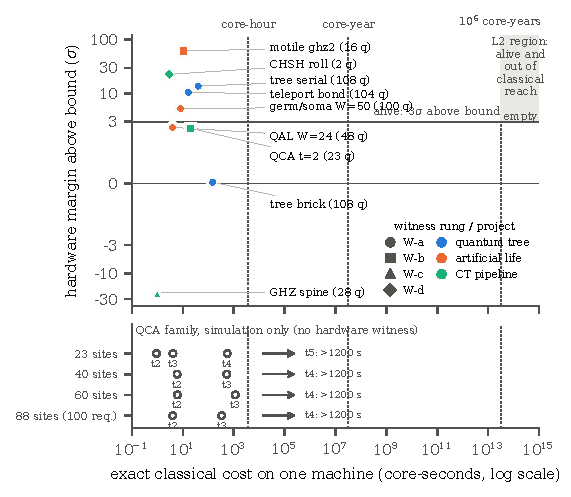
\includegraphics[width=\columnwidth]{fig1_map.pdf}
\caption{\figOneCaption}
\label{fig:map}
\end{figure}

\begin{table}[t]
\centering
\caption{Exact classical cost of the QCA Z snapshot (ideal, exact MPS, one eight-core machine) by patch size and
depth. Rows with $>$ did not finish within the stated limit (1200~s wall clock, 20~GB address space).}
\label{tab:scan}
\small
\begin{tabular}{rrrrr}
\toprule
sites (req./alloc.) & $t$ & 2q gates & $\chi$ & exact (s)\\
\midrule
23/23 & 2 & 92 & 13 & 0.11\\
23/23 & 3 & 138 & 45 & 0.51\\
23/23 & 4 & 184 & 492 & 68.53\\
23/-- & 5 & -- & -- & $>1200$\\
40/40 & 2 & 160 & 26 & 0.74\\
40/40 & 3 & 240 & 256 & 66.08\\
40/-- & 4 & -- & -- & $>1200$\\
60/60 & 2 & 244 & 52 & 0.76\\
60/60 & 3 & 366 & 482 & 143.56\\
60/-- & 4 & -- & -- & $>1200$\\
100/88 & 2 & 356 & 16 & 0.49\\
100/88 & 3 & 534 & 144 & 41.96\\
100/-- & 4 & -- & -- & $>1200$\\
\bottomrule
\end{tabular}

\end{table}

Beyond these layers, the routes that could make quantum models useful for medical prediction, such as rare-event
estimation and drug--target chemistry, need fault-tolerant hardware and lie outside this record~\cite{babbush2021,
cordier2022}.

\section{What does not work yet: simulating life}\label{sec:life}
Our first two projects tried to make quantum hardware simulate living processes: a 108-qubit genome that grows a
tree, with a feedback rule between generations and an optional teleported long-range bond, and a faithful
operator-by-operator rebuild of quantum artificial life~\cite{alvarez2018}. The rebuild covers founder, clone,
mutation, phenotype, aging death and interaction, plus germ/soma and motile variants.

\textbf{Method.} For every hardware result we rebuilt the logical circuit from the original builder and simulated it
exactly with Qiskit Aer 0.17.2 on one eight-core machine with 31~GB of memory. We used a matrix product state (MPS)
without truncation, or a stabilizer or statevector simulation where cheaper. We record the wall-clock time, the maximal
MPS bond dimension $\chi$ and the ideal value of the observable the hardware reported. Quantum-tree generation~0 is
fixed by its seed; later generations are replayed exactly from the recorded frequencies where noted.

\begin{table*}[t]
\centering
\caption{Hardware results and their exact classical reproduction on one eight-core machine. Hardware and ideal values are the reported observable (tree: $c(1)$ at generation 0, bond: mean bond $c(d)$; QAL: $\langle X^{\otimes W}\rangle$; ghz2: $\langle XX\rangle+\langle ZZ\rangle$; GHZ: fidelity; QCA: pair negativity). Cost: wall clock for the exact state plus samples. Backends: \texttt{ibm\_kingston} (tree serial and brick, QAL), \texttt{ibm\_marrakesh} (bond, motile, CT roll, D-SCALE).}
\label{tab:record}
\begin{tabular}{lrcrrrrl}
\toprule
Circuit & qubits & rung & hardware & ideal & cost (s) & $\chi$ & verdict\\
\midrule
Tree, serial, 2 layers & 108 & W-a & $-$0.104 & $-$0.157 & 5.00 & 4 & real, cheap\\
Tree, floor (1 layer) & 108 & W-a & +0.024 & +0.0008 & 0.68 & 1 & artefact\\
Tree, brick wall, 2 layers & 108 & W-a & $-$0.030 & $-$0.045 & 18.26 & 8 & real, cheap\\
QAL Month 4, $W=24$ & 48 & W-a & 0.038 & 0.767 & 0.49 & 2 & alive $2.4\sigma$\\
QAL germ/soma, $W=50$ & 100 & W-a & 0.058 & 1.000 & 1.00 & 2 & alive 5.2$\sigma$\\
QAL motile, ghz2 & 16 & W-b & 1.959 & 2.000 & 1.30 & -- & certified\\
CT roll, CHSH & 2 & W-d & 2.733 & 2.828 & 0.37 & -- & 22.7$\sigma$ $>2$\\
D-SCALE GHZ spine & 28 & W-c & 0.055 & 1.000 & 0.12 & 2 & fails 0.5\\
D-SCALE QCA, $t=2$ & 23 & W-b & 0.014 & $-$- & 2.42 & 96 & marginal\\
\bottomrule
\end{tabular}
\end{table*}


\textbf{Every result is classically cheap.} Every circuit in Table~\ref{tab:record} is reproduced exactly in at most
\costMaxS{}~s, with $\chi\le\chiMaxRecord{}$. The genealogy circuits are the extreme case. The 100-qubit germ/soma
circuit at $W=50$ has $\chi=2$ and is sampled in \costPjFifty{}~s, and the same construction at 154 qubits ($W=77$,
the full chip) takes \costPjSevenSeven{}~s at $\chi=2$. Hardware retained \pjFiftyRetainPct{}\% of the ideal witness
at $W=50$ and \mFourTwentyFourRetainPct{}\% at $W=24$ (Table~\ref{tab:qal}).

\begin{table}[t]
\centering
\caption{Genealogy witness $\langle X^{\otimes W}\rangle$ on \texttt{ibm\_kingston} against its exact ideal and
the exact classical cost (one eight-core machine, MPS, $\chi=2$ in every row). Month~4: three repeats, mutation
scale 0.08 (hardware angles from a certified entropy service; ideal with pseudo-random angles of the same scale).
Germ/soma: one run per width, no mutation; steps grow with $W$. W-a rung.}
\label{tab:qal}
\scriptsize
\setlength{\tabcolsep}{3pt}
\begin{tabular}{lrrrrrrr}
\toprule
Model & $W$ & qubits & steps & hardware & $k\sigma$ & ideal & exact (s)\\
\midrule
Month 4 & 3 & 6 & 3 & 0.879 & 33.0 & 0.975 & 0.07\\
Month 4 & 4 & 8 & 3 & 0.808 & 38.3 & 0.954 & 0.09\\
Month 4 & 6 & 12 & 3 & 0.612 & 42.2 & 0.931 & 0.13\\
Month 4 & 12 & 24 & 3 & 0.301 & 17.8 & 0.883 & 0.25\\
Month 4 & 24 & 48 & 3 & 0.038 & 2.4 & 0.767 & 0.49\\
Month 4 & 32 & 64 & 3 & 0.008 & 0.6 & 0.718 & 0.65\\
\midrule
germ/soma & 4 & 8 & 4 & 0.899 & 81.4 & 1.000 & 0.09\\
germ/soma & 6 & 12 & 4 & 0.870 & 78.8 & 1.000 & 0.12\\
germ/soma & 12 & 24 & 6 & 0.756 & 68.4 & 1.000 & 0.24\\
germ/soma & 16 & 32 & 8 & 0.296 & 26.8 & 1.000 & 0.57\\
germ/soma & 24 & 48 & 12 & 0.193 & 17.5 & 1.000 & 0.49\\
germ/soma & 28 & 56 & 14 & 0.355 & 32.2 & 1.000 & 1.25\\
germ/soma & 32 & 64 & 16 & 0.271 & 24.5 & 1.000 & 1.65\\
germ/soma & 36 & 72 & 18 & 0.220 & 19.9 & 1.000 & 1.24\\
germ/soma & 40 & 80 & 20 & 0.067 & 6.1 & 1.000 & 1.46\\
germ/soma & 42 & 84 & 21 & 0.068 & 6.2 & 1.000 & 1.78\\
germ/soma & 46 & 92 & 23 & 0.081 & 7.3 & 1.000 & 1.83\\
germ/soma & 50 & 100 & 25 & 0.058 & 5.2 & 1.000 & 1.00\\
\bottomrule
\end{tabular}

\end{table}

\textbf{Nine checks we learned the hard way.} Table~\ref{tab:audit} lists nine ways a result can look quantum without
being so. Each one is an instance in our own record, with the number that exposed it and the test that catches it.
Three changed our conclusions.

\begin{table*}[t]
\centering
\caption{Nine checks every quantum-biology result should pass. Each row is an instance in our own hardware
record where a check failed, the number that showed it, and the test that catches it.}
\label{tab:audit}
\small
\begin{tabular}{p{0.3cm}p{2.9cm}p{4.3cm}p{5.0cm}p{3.6cm}}
\toprule
& Check fails when & Instance in our record & Number & Test that catches it\\
\midrule
F1 & Single-basis biology read as quantum & QAL phenotype populations, alive counts & classical surrogate matches the
quantum phenotype to \surrUnitaryFixed{} (unitary death); the shipped surrogate had a SWAP-order bug
(\surrUnitaryCode{}) and a mis-set damping form (\surrDamp{}) & build the classical surrogate of the same
probabilities\\
F2 & Diversity or entropy as evidence & tree art metric (mean bit entropy) & diversity \qtDivHw{} (hardware) vs
\qtDivSim{} (classical surrogate) while $c(1)$ differs by $|z|=\qtZsim$ & measure multi-qubit correlations\\
F3 & Null that excludes too little & tree ``no-entangler'' floor; QAL measure-and-resend null & floor depth
\qtDepthFloor{} equals one-layer depth \qtDepthLone{}; a separable mixture scores $\langle X^{\otimes W}\rangle=1$ &
a real no-op control; the separable set as null\\
F4 & Depth or crosstalk confound & tree floor arm & ideal product state ($\chi=1$, $c(1)=\qtIdealLoneMean$), hardware
$c(1)=\qtHwLoneMean$ & exact ideal of the same circuit\\
F5 & One-basis witness & QAL $W=24$ and $W=50$ & only $\langle X^{\otimes W}\rangle$ measured; the one GME test
(28 qubits) gave $F=\ghzF<0.5$ & two-setting GME witness~\cite{toth2005}\\
F6 & Entangled taken as hard & GHZ spine, all genealogies & $\chi=2$ for every genealogy circuit up to 154 qubits
& stabilizer, MPS, BP simulation\\
F7 & Hilbert-space size taken as hardness & ``$2^{108}$ amplitudes'' for the 108-qubit tree & exact at
$\chi\le\qtChiLfour$, at most \qtCostLfour{}~s & the cheapest exact method, not the state vector\\
F8 & Logical depth or qubit count as merit & teleport vs SWAP; 9-qubit roll & \teleportAuditCell{}; roll compiles
from \rollTwoQLogical{} to \rollTwoQIsa{} two-qubit gates & exact replay; compiled two-qubit count\\
F9 & Simulated certification & CHSH in simulation & only the hardware job certifies: $S=\chshS\pm\chshSig$
& Bell test on hardware in the same job\\
\bottomrule
\end{tabular}
\end{table*}


\emph{A control that was not a control.} The quantum-tree study subtracted a ``no-entangler'' hardware floor run with
zero entangling layers. The circuit builder loops \texttt{for \_ in range(max(1, layers))}, so the floor run applied
one full entangling layer. The recorded logical depth confirms it: \qtDepthFloor{} for the floor against
\qtDepthLone{} for one layer. One serial layer leaves the generation-0 state an exact product state ($\chi=1$, ideal
$c(1)=\qtIdealLoneMean{}$), yet the hardware read $c(1)=\qtHwLoneMean{}$, a device artefact. The two-layer arm is a
genuine circuit correlation (ideal \qtIdealLtwoMin{} to \qtIdealLtwoMax{}, hardware \qtHwLtwoMean{}), reproduced
classically at $\chi=4$ in \qtCostLtwo{}~s, and the shallow brick-wall layout tracks its ideal closely (ideal
\bwIdealLoneMean{}, hardware \bwHwLoneMean{}).

\emph{A one-basis witness.} The genealogy signal $\langle X^{\otimes W}\rangle-\prod_i\langle X_i\rangle$ is compared
with a measure-and-resend surrogate, which gives zero. The fully separable mixture
$\tfrac12(|{+}\rangle\langle{+}|^{\otimes W}+|{-}\rangle\langle{-}|^{\otimes W})$ gives $\langle X^{\otimes
W}\rangle=1$ and $\prod_i\langle X_i\rangle=0$ for even $W$. The $W=24$ and $W=50$ results are therefore W-a
correlations, not entanglement certificates, which is why Layer~2 of the road needs the two-setting witness.

\emph{Depth is not the figure of merit.} \teleportParagraph

\textbf{What survived as a design rule.} Dissipative death that entangles the phenotype with the genotype removes
the genealogy signal: at one step it is alive at $W=9$ ($k=\dampNineK\sigma$) and dead at $W=10$ ($k=\dampTenK\sigma$).
Severing that coupling restores it, from \pjEntNat{} to \pjSepNat{} at $W=4$. Both arms use the same test on the same
processor, so the result holds whatever the witness rung. This is the building block of Layer~2.

\section{Why faithful life simulations are classically easy}\label{sec:easy}
The record shows one pattern from three sides.

\emph{P1 (diagonal biology).} Clone (CNOT), metabolism (Toffoli), phenotype copy, SWAP interaction and amplitude
damping map computational-basis states to basis states or act as stochastic maps on them. After a product-state
preparation, such circuits have single-basis statistics given by a classical Markov chain. With the circuit's SWAP
order replayed, our classical surrogate matches the quantum phenotype to \surrUnitaryFixed{} (unitary death).

\emph{P2 (genealogies are trees).} In a clone cascade each new individual interacts once with its parent. Any
bipartition of the line is crossed by the state of one qubit, which bounds the Schmidt rank by 2.
Tensor-network contraction cost is exponential only in the treewidth~\cite{markov2008}, and low-$\chi$ states are
efficiently simulable~\cite{vidal2003}. We measured $\chi=2$ for every genealogy circuit from $W=3$ to $77$.

\emph{P3 (equilibrium is stoquastic).} The mutation--selection equilibrium of the quasispecies model is the ground
state of an Ising chain in a transverse field: mutation plays the field and fitness the coupling~\cite{baake1997}.
That Hamiltonian is sign-free, the regime where classical Monte Carlo usually works.

\textbf{Not worth pursuing now.} From P1--P3 and the record:
(a)~quantum life or tumour-evolution simulation as a predictor, since every faithful circuit we ran is reproduced
classically in at most \costMaxS{}~s;
(b)~population statistics (cell counts, growth curves, lifetimes) as quantum evidence, since they are single-basis;
(c)~qubit count as a headline for tree-shaped genealogies, since $\chi$ stays 2 at any width;
(d)~logical depth as the argument for a routing scheme, since only an exact replay decides.
What remains open, and what Layer~4 measures, is the one exit the propositions leave: interactions that close
loops, combined with non-Clifford coupling.

\section{Threats to validity}
Most hardware configurations ran once (N=1); the Month-4 width sweep and the quantum-tree arms used three
repeats. Classical costs are wall-clock times on one eight-core machine, an upper bound on the classical cost of
each circuit, not a lower bound on classical hardness. A BP-hard flag on a small patch is not classical hardness,
since exact simulation of that patch takes seconds. The noise model (FakeMarrakesh) is a published calibration
snapshot, not the calibration of the day. All CT cases share one host scan, and the roll and seed comparisons rest
on twelve tumours from one job. Replays assume the recorded random stream; the environment schedule matched the
recorded one in every generation we replayed.

\section{Conclusion}
\conclusionParagraph

\section*{Data and code availability}
All hardware run files, the exact-simulation scripts and the generators of every number and table in this paper
are in the author's repository (\texttt{THESIS/QuantumEvolutionFrontier/analysis}). Every number in the paper is
written by \texttt{paper\_numbers.py} from those files.

\bibliographystyle{IEEEtran}
\bibliography{refs}

\end{document}
